% linkedin_article_part2.tex — Quant Risk Engine: Part 2 Technical Article
% Author: Pop Gabriel-Răzvan | March 2026
% Compile: tectonic linkedin_article_part2.tex

\documentclass[11pt,a4paper]{article}

% --- Packages ---
\usepackage[utf8]{inputenc}
\usepackage[T1]{fontenc}
\usepackage{lmodern}
\usepackage{amsmath,amssymb,amsthm}
\usepackage{graphicx}
\usepackage{booktabs}
\usepackage[colorlinks=true,linkcolor=accentblue,urlcolor=accentblue,citecolor=accentblue]{hyperref}
\usepackage[dvipsnames]{xcolor}
\usepackage[margin=1in]{geometry}
\usepackage{enumitem}
\usepackage{float}
\usepackage{caption}
\usepackage{subcaption}
\usepackage{fancyhdr}
\usepackage{titlesec}
\usepackage{microtype}

% --- Color scheme ---
\definecolor{accentblue}{RGB}{0,70,140}

% --- Section formatting ---
\titleformat{\section}{\Large\bfseries\color{accentblue}}{\thesection.}{0.5em}{}
\titleformat{\subsection}{\large\bfseries\color{accentblue!80!black}}{\thesubsection}{0.5em}{}

% --- Paragraph spacing ---
\setlength{\parindent}{0pt}
\setlength{\parskip}{0.8em}

% --- Header/footer ---
\pagestyle{fancy}
\fancyhf{}
\fancyhead[L]{\small\textcolor{gray}{Pop Gabriel-R\u{a}zvan}}
\fancyhead[R]{\small\textcolor{gray}{Building a Quant Risk Engine --- Part 2}}
\fancyfoot[C]{\small\thepage}
\renewcommand{\headrulewidth}{0.4pt}

% --- Document ---
\begin{document}

% ===== TITLE BLOCK =====
\begin{center}
    {\LARGE\bfseries\color{accentblue} Building a Quant Risk Engine from Scratch --- Part 2:\\[4pt]
    When Diversification Fails and Models Lie}

    \vspace{0.6em}
    {\large Sobol QMC, Vine Copulas, Walk-Forward Backtesting,\\
    and the Dollar Cost of Model Risk}

    \vspace{1em}
    {\large Pop Gabriel-R\u{a}zvan}\\[4pt]
    {\normalsize March 2026}
\end{center}

\vspace{0.5em}

\begin{abstract}
\noindent
In Part~1, we built a stochastic volatility simulation engine and showed that Expected Shortfall estimates diverge by 30\% across volatility models. Part~2 puts this engine to work. We demonstrate 191$\times$ convergence improvement via Sobol quasi-Monte Carlo, show that equity tail dependence jumps from 0.01 to 0.49 during crises using vine copulas, validate on 1{,}053 days of real market data where Heston passes Basel traffic-light tests that GBM fails, and quantify that a Black--Scholes hedger underestimates tail losses by 6--12$\times$ under realistic stochastic volatility. An interactive dashboard is available at \url{https://quantriskeng.streamlit.app}.
\end{abstract}

\vspace{0.3em}
\hrule
\vspace{1em}

% ===== SECTION 1 =====
\section{Faster Convergence --- Quasi-Monte Carlo with Variance Reduction}

Standard Monte Carlo converges at $O(N^{-1/2})$---halving the error requires quadrupling the paths. For Expected Shortfall at the 99th percentile, where only 1\% of simulated paths contribute to the estimate, this inefficiency is compounded: the effective sample size for the tail is $N/100$, and the resulting estimator has high variance. In production risk systems where ES must be computed across thousands of positions daily, convergence speed is not a theoretical nicety but a computational bottleneck.

Sobol sequences replace pseudorandom samples with low-discrepancy quasi-random numbers that fill the unit hypercube more uniformly. The theoretical convergence rate improves from the Monte Carlo $O(N^{-1/2})$ to:
\begin{equation}
\varepsilon_{\text{QMC}} \sim O\!\left(N^{-1} (\log N)^d\right)
\end{equation}
where $d$ is the effective dimension. For smooth integrands, this approaches $O(N^{-1})$---achieving the same precision with the square root of the computational effort. We implement the Joe--Kuo direction numbers~\cite{joe2010} with Brownian bridge path construction, which concentrates the most important dimensions (terminal value, early time steps) onto the lowest-discrepancy Sobol coordinates.

We supplement QMC with two classical variance reduction techniques. \textit{Antithetic variates} exploit the symmetry of the standard normal distribution: for each path driven by innovations $Z_1, \ldots, Z_n$, we simulate a mirror path using $-Z_1, \ldots, -Z_n$, halving the variance of symmetric functionals. \textit{Control variates} use GBM---which has a known analytical solution---as a control for Heston:
\begin{equation}
\hat{\mu}_{\text{CV}} = \hat{\mu}_{\text{Heston}} + c^* \left( \mathbb{E}[g_{\text{GBM}}] - \hat{g}_{\text{GBM}} \right), \quad
c^* = -\frac{\text{Cov}(\hat{Y}, \hat{G})}{\text{Var}(\hat{G})}
\end{equation}
where both models are driven by identical random numbers. The achieved correlation of $\rho = 0.69$ reflects the fundamental difference between the models---as model risk increases, the GBM control becomes less effective. This is itself a diagnostic: the control variate correlation quantifies how far the stochastic volatility model has departed from the constant-volatility assumption.

\begin{table}[H]
\centering
\begin{tabular}{lc}
\toprule
\textbf{Technique} & \textbf{Improvement} \\
\midrule
Sobol QMC (mean estimation)          & 191$\times$ lower standard error \\
Sobol QMC (ES estimation)            & $\sim$1.5$\times$ faster convergence \\
Control Variates (GBM$\to$Heston)    & 28\% SE reduction ($\rho = 0.69$) \\
Antithetic Variates                  & 80\% SE reduction \\
\bottomrule
\end{tabular}
\caption{Variance reduction results. Sobol QMC provides the largest gain for smooth statistics (mean, variance), while antithetic variates are most effective for tail risk metrics.}
\label{tab:variance_reduction}
\end{table}

\begin{figure}[H]
\centering
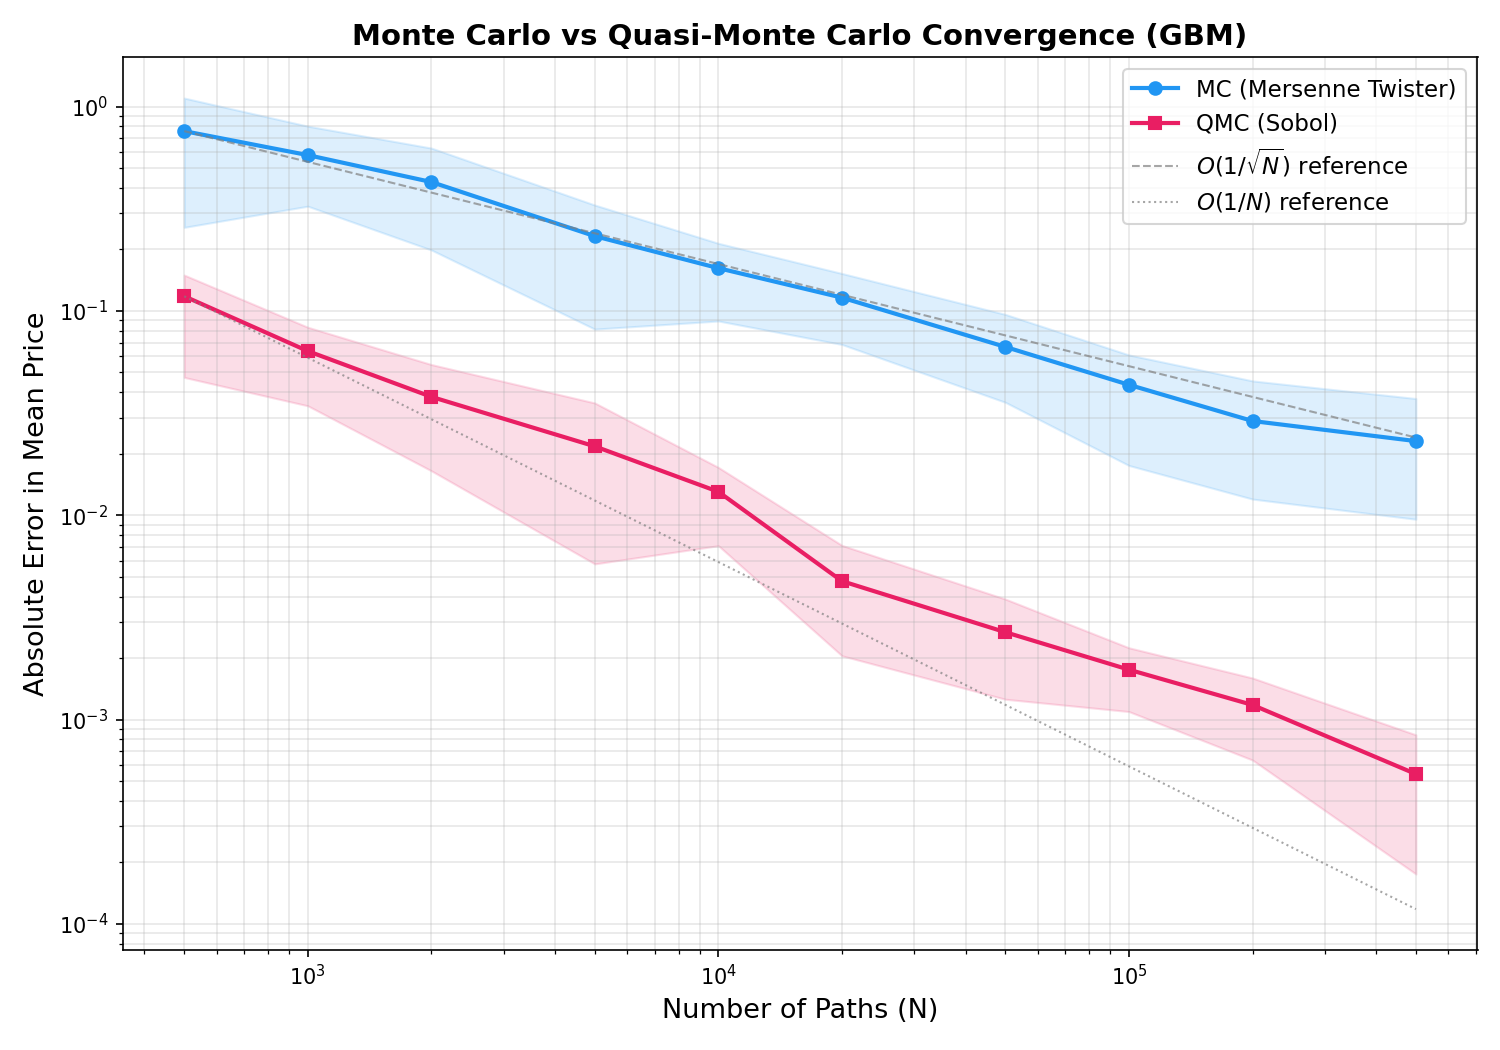
\includegraphics[width=0.95\textwidth]{figures/convergence_comparison.png}
\caption{Convergence comparison: standard Monte Carlo (blue) vs.\ Sobol quasi-Monte Carlo (red). On log-log scale, MC follows the theoretical $O(N^{-1/2})$ slope while QMC achieves near-$O(N^{-1})$ convergence, requiring orders of magnitude fewer paths for equivalent precision.}
\label{fig:convergence}
\end{figure}

% ===== SECTION 2 =====
\section{When Diversification Fails --- Vine Copulas and Tail Dependence}

The most dangerous assumption in portfolio risk management is not about individual assets---it is about how they move together. In our empirical analysis (Part~1), we documented that equity pair correlations jump from 0.04--0.08 in calm markets to 0.37--0.42 during crashes. Pearson correlation cannot capture this asymmetry because it measures linear, symmetric dependence. A portfolio that appears well-diversified under normal conditions can become concentrated precisely when diversification matters most.

\subsection{Copulas --- Separating Margins from Dependence}

Sklar's theorem~\cite{sklar1959} provides the mathematical foundation for modeling dependence independently of marginal distributions:
\begin{equation}
F(x_1, \ldots, x_d) = C\!\left(F_1(x_1), \ldots, F_d(x_d)\right)
\end{equation}
The copula $C$ captures the pure dependence structure, independent of how each individual asset's returns are distributed. This separation is powerful: we can combine stochastic volatility marginals (from our C++ simulation engine) with realistic multivariate tail dependence (from the copula), without forcing either component to compromise.

\subsection{Vine Copulas --- Flexible High-Dimensional Dependence}

For $d = 6$ assets (SPY, IBM, JPM, AAPL, TLT, GLD), specifying a full $d$-dimensional copula directly is impractical. Vine copulas~\cite{aas2009} decompose the multivariate problem into a cascade of bivariate copulas arranged in a tree structure. Each bivariate pair is modeled with a Student-$t$ copula that captures both upper and lower tail dependence, and the tree structure is selected automatically by maximizing Kendall's $\tau$ across levels.

The key advantage over Gaussian copulas is the ability to model \textit{asymmetric tail dependence}: the probability that two assets crash simultaneously can differ from the probability that they both surge. For equity portfolios, lower tail dependence systematically exceeds upper tail dependence---diversification erodes in crashes but not in rallies.

\begin{table}[H]
\centering
\begin{tabular}{lc}
\toprule
\textbf{Finding} & \textbf{Value} \\
\midrule
Vine Copula ES$_{99}$ (equal weight)          & 4.34\% \\
Gaussian Copula ES$_{99}$                     & 3.78\% (underestimates by 15\%) \\
Independent ES$_{99}$                         & 2.62\% \\
JPM risk contribution                         & 38.1\% of ES from 16.7\% allocation \\
TLT risk contribution                         & $-$2.3\% (crash hedge) \\
Crisis tail dependence (equity pairs)         & $\lambda_L$ jumps from 0.01 to 0.49 \\
\bottomrule
\end{tabular}
\caption{Portfolio risk under vine copula dependence. JPM contributes 2.3$\times$ its weight to tail risk; TLT provides genuine diversification even during crises.}
\label{tab:copula}
\end{table}

The Euler allocation decomposes portfolio ES into additive per-asset contributions:
\begin{equation}
\text{ES}_i = \mathbb{E}\!\left[ w_i\, r_i \;\middle|\; r_{\text{portfolio}} \leq -\text{VaR}_\alpha \right], \quad \sum_{i=1}^{d} \text{ES}_i = \text{ES}_{\text{portfolio}}
\end{equation}
The results are striking. Despite holding only one-sixth of the portfolio, JPM contributes 38.1\% of tail risk because it is highly correlated with other equities in the left tail. SPY and AAPL contribute 21.2\% and 22.6\% respectively. GLD provides marginal diversification (2.3\% contribution from 16.7\% weight). TLT contributes \textit{negatively} ($-$2.3\%)---it is the only asset that genuinely hedges portfolio tail risk, because bonds tend to rally during equity crashes.

\begin{figure}[H]
\centering
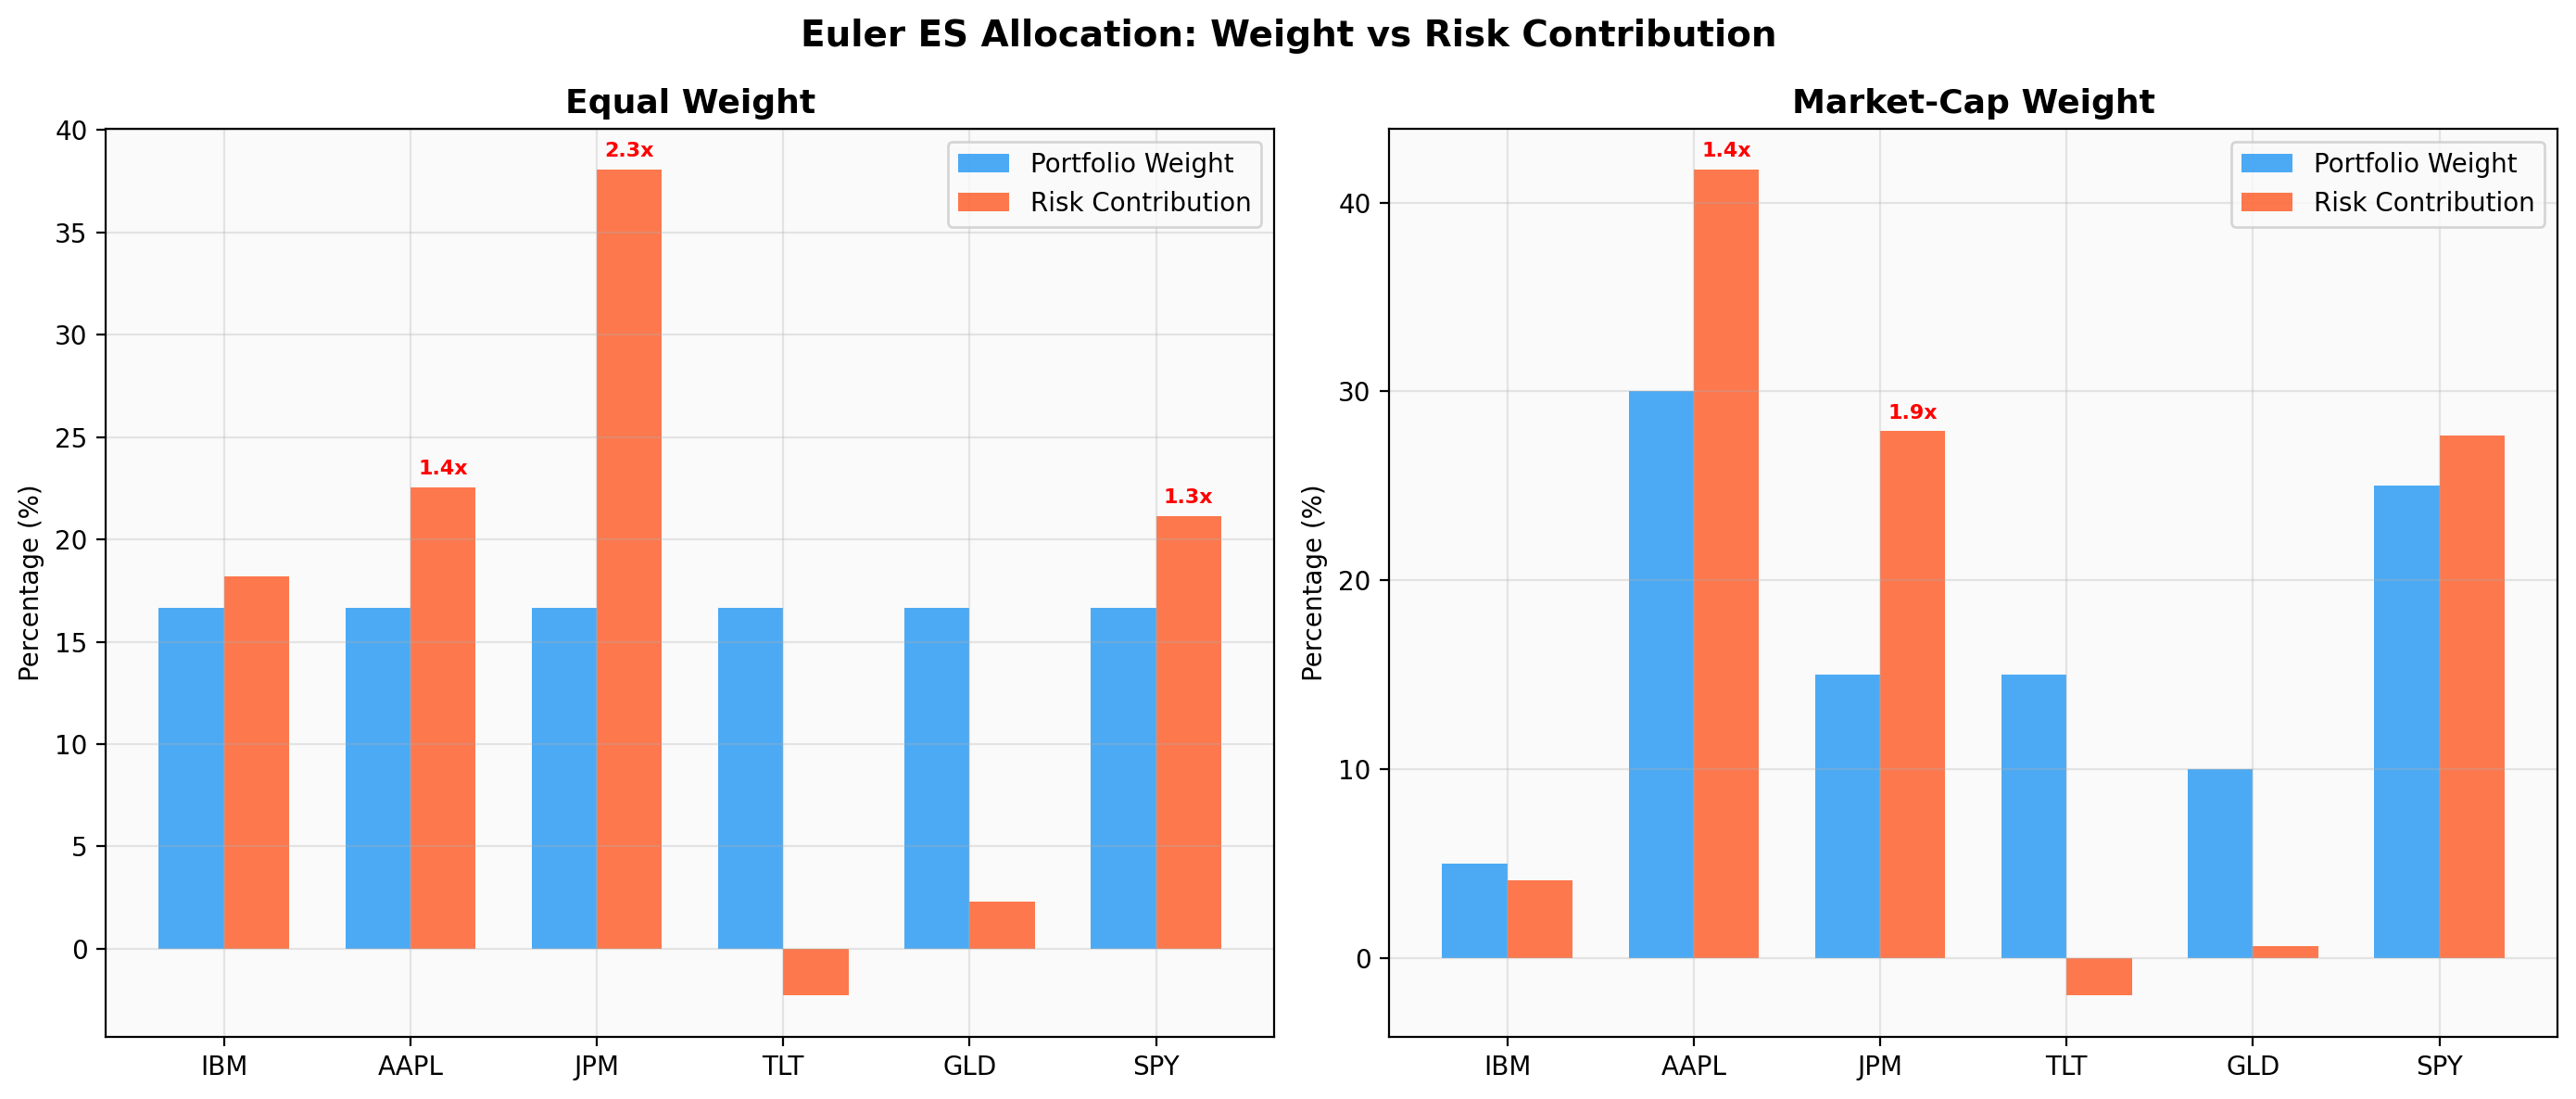
\includegraphics[width=0.95\textwidth]{figures/euler_allocation.png}
\caption{Euler risk allocation under vine copula. Left: portfolio weights (equal, 16.7\% each). Right: ES$_{99}$ contributions. JPM dominates tail risk at 38.1\%; TLT provides a negative contribution (diversification benefit that persists in crashes).}
\label{fig:euler}
\end{figure}

\begin{figure}[H]
\centering
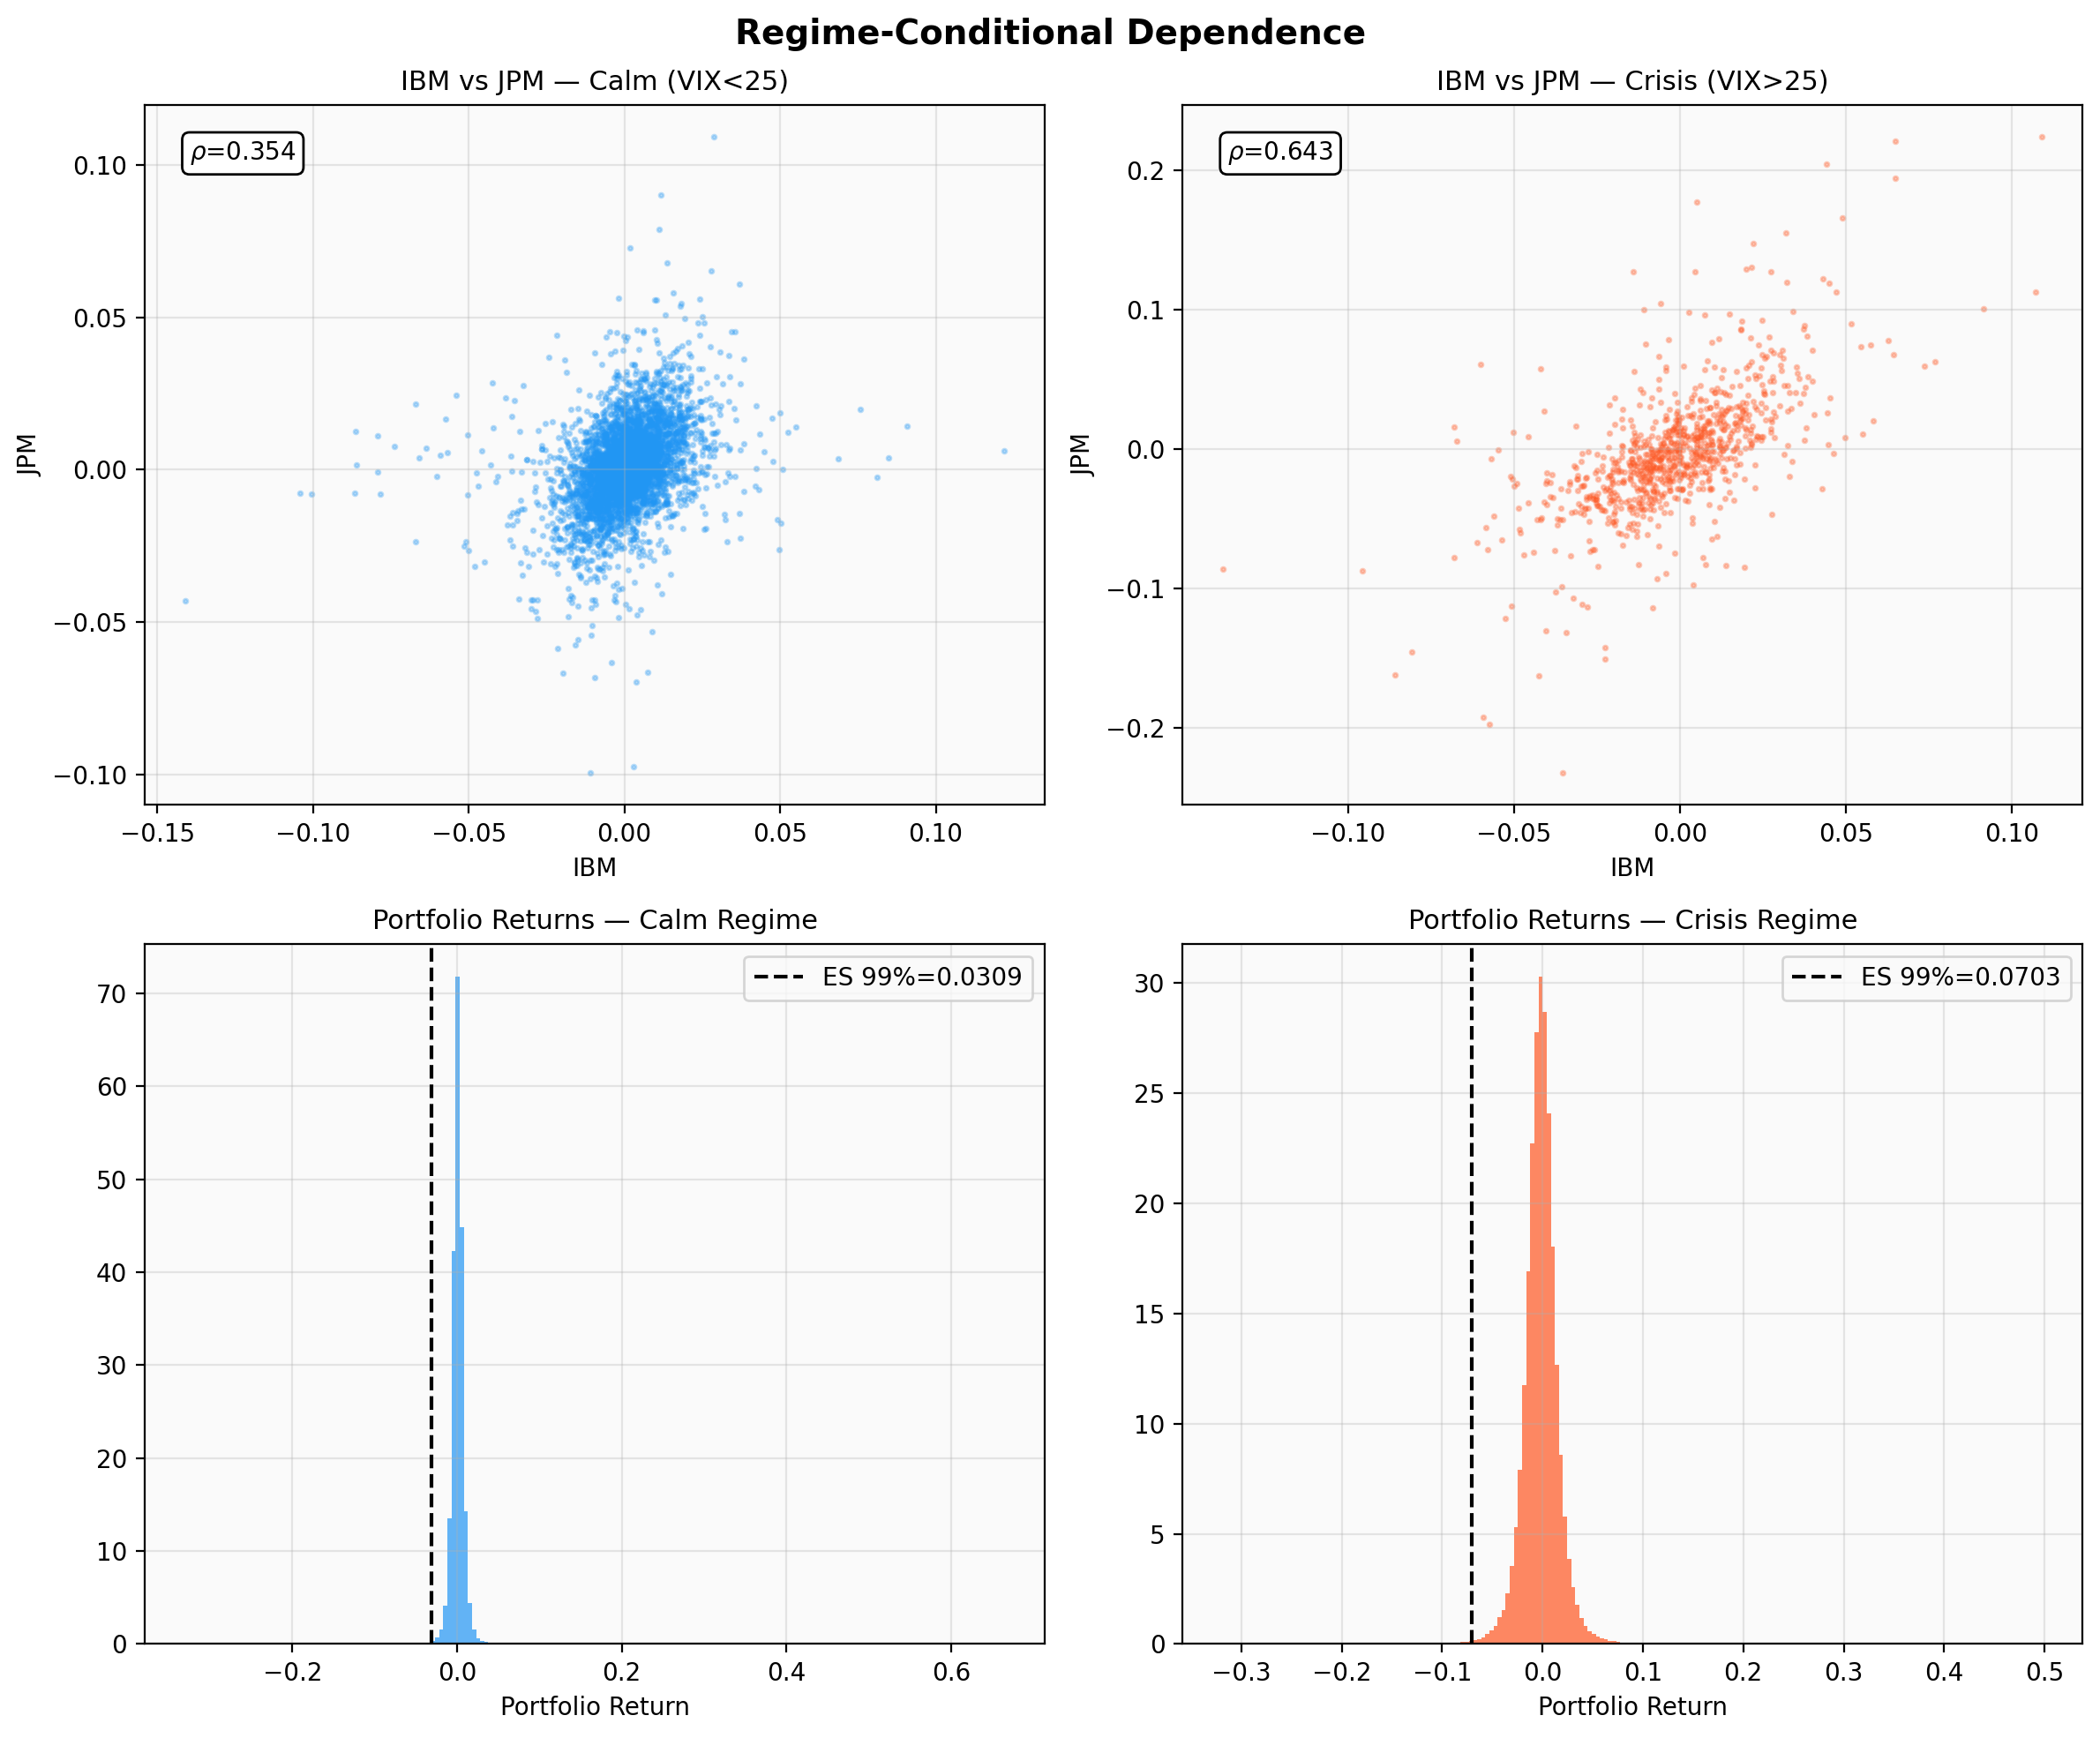
\includegraphics[width=0.95\textwidth]{figures/regime_dependence.png}
\caption{Tail dependence across market regimes. During calm periods (left), equity tail dependence $\lambda_L$ is near zero (0.01--0.27). During crises (right), it jumps to 0.42--0.52 for equity pairs---a regime shift that Gaussian copulas cannot capture.}
\label{fig:regime_dependence}
\end{figure}

% ===== SECTION 3 =====
\section{Proof on Real Data --- Walk-Forward Backtesting}

Theory and simulation are necessary but not sufficient. The critical question is whether our models produce calibrated risk estimates on \textit{real market data}---data the models have never seen during calibration.

\subsection{Setup}

We run a 1{,}053-day walk-forward backtest (2022--2025) on SPY, IBM, and JPM. At each date $t$, we calibrate model parameters on all data prior to $t$, simulate 100{,}000 one-day-ahead scenarios, and compute VaR$_{99}$. We then compare with the realized return on day $t+1$. Parameters are recalibrated via differential evolution every 60 trading days; the current variance $v_0$ is updated daily from a 20-day realized volatility window. This mimics how a production risk system would operate: periodic full recalibration with daily state updates.

\subsection{Statistical Tests}

The Kupiec test~\cite{kupiec1995} evaluates \textit{unconditional coverage}---whether the observed exceedance rate matches the target:
\begin{equation}
LR_{UC} = -2 \ln \frac{(1-p)^{T-x}\, p^x}{(1-\hat{p})^{T-x}\, \hat{p}^x} \sim \chi^2(1)
\end{equation}
where $p$ is the target exceedance rate, $\hat{p} = x/T$ is the observed rate, and $x$ is the number of exceedances over $T$ days.

The Christoffersen test~\cite{christoffersen1998} extends this to \textit{conditional coverage}, testing whether exceedances are independent over time. It constructs the transition matrix of exceedance sequences and tests whether $P(\text{exceed}_{t+1} \mid \text{exceed}_t) = P(\text{exceed}_{t+1} \mid \text{no exceed}_t)$. Exceedance clustering indicates systematic model failure---the model is overconfident precisely during high-volatility regimes.

\subsection{Results}

\begin{table}[H]
\centering
\begin{tabular}{lccccc}
\toprule
\textbf{Model} & \textbf{Exceedances} & \textbf{Rate} & \textbf{Kupiec $p$} & \textbf{Christ.\ $p$} & \textbf{Basel Zone} \\
\midrule
ARIMA         & 15 & 1.43\% & 0.193 (pass) & 0.023 (fail) & GREEN \\
GBM           & 22 & 2.09\% & 0.002 (fail) & 0.002 (fail) & YELLOW \\
Heston        & 14 & 1.33\% & 0.306 (pass) & 0.237 (pass) & GREEN \\
Rough Heston  & 14 & 1.33\% & 0.306 (pass) & 0.237 (pass) & GREEN \\
\bottomrule
\end{tabular}
\caption{Walk-forward VaR$_{99}$ backtest on SPY (1{,}053 trading days). Expected exceedances under correct calibration: $\approx$10.5. GBM is formally rejected by Kupiec; ARIMA passes Kupiec but fails Christoffersen (clustered violations).}
\label{tab:backtest}
\end{table}

GBM produces 22 exceedances where approximately 10.5 are expected---formally rejected by Kupiec ($p = 0.002$). Its VaR is systematically too narrow because constant volatility cannot adapt to regime changes. ARIMA achieves acceptable unconditional coverage (15 exceedances, $p = 0.193$) but fails the Christoffersen independence test ($p = 0.023$) with a clustering ratio of 10.6$\times$. Its violations come in bursts during volatile periods---arguably more dangerous than a uniform over-count, because clustered violations can compound into catastrophic multi-day losses.

Heston and Rough Heston both achieve Basel GREEN with 14 exceedances (1.33\% vs.\ 1\% target) and pass both Kupiec and Christoffersen tests. They succeed because the stochastic variance process adapts to regime changes: when realized volatility rises, $v_0$ is updated upward, widening the one-day VaR. The models are not perfect---14 exceedances is still above the expected 10.5---but they are statistically indistinguishable from correct calibration.

\subsection{Regime Analysis}

The regime decomposition reveals where models fail most dramatically:

\begin{table}[H]
\centering
\begin{tabular}{lcccc}
\toprule
\textbf{Model} & \textbf{Calm Rate} & \textbf{Crisis Rate} & \textbf{Crisis Days} & \textbf{Target} \\
\midrule
ARIMA         & 0.00\% & 9.32\% & 161 & 1\% \\
GBM           & 0.22\% & 12.42\% & 161 & 1\% \\
Heston        & 0.45\% & 6.21\% & 161 & 1\% \\
Rough Heston  & 0.45\% & 6.21\% & 161 & 1\% \\
\bottomrule
\end{tabular}
\caption{VaR$_{99}$ exceedance rates by market regime. All models struggle in crisis periods (target: 1\%), but Heston halves GBM's crisis exceedance rate from 12.4\% to 6.2\%.}
\label{tab:regime}
\end{table}

GBM's crisis exceedance rate of 12.4\% means that on roughly one in eight crisis days, losses exceed the stated VaR---over twelve times the target rate. ARIMA is even more extreme in its failure mode: zero exceedances during calm periods (overfitting) followed by 9.3\% during crises. Heston reduces the crisis rate to 6.2\%---still elevated, but halved relative to GBM. The improvement comes directly from the variance process adapting to regime changes.

\begin{figure}[H]
\centering
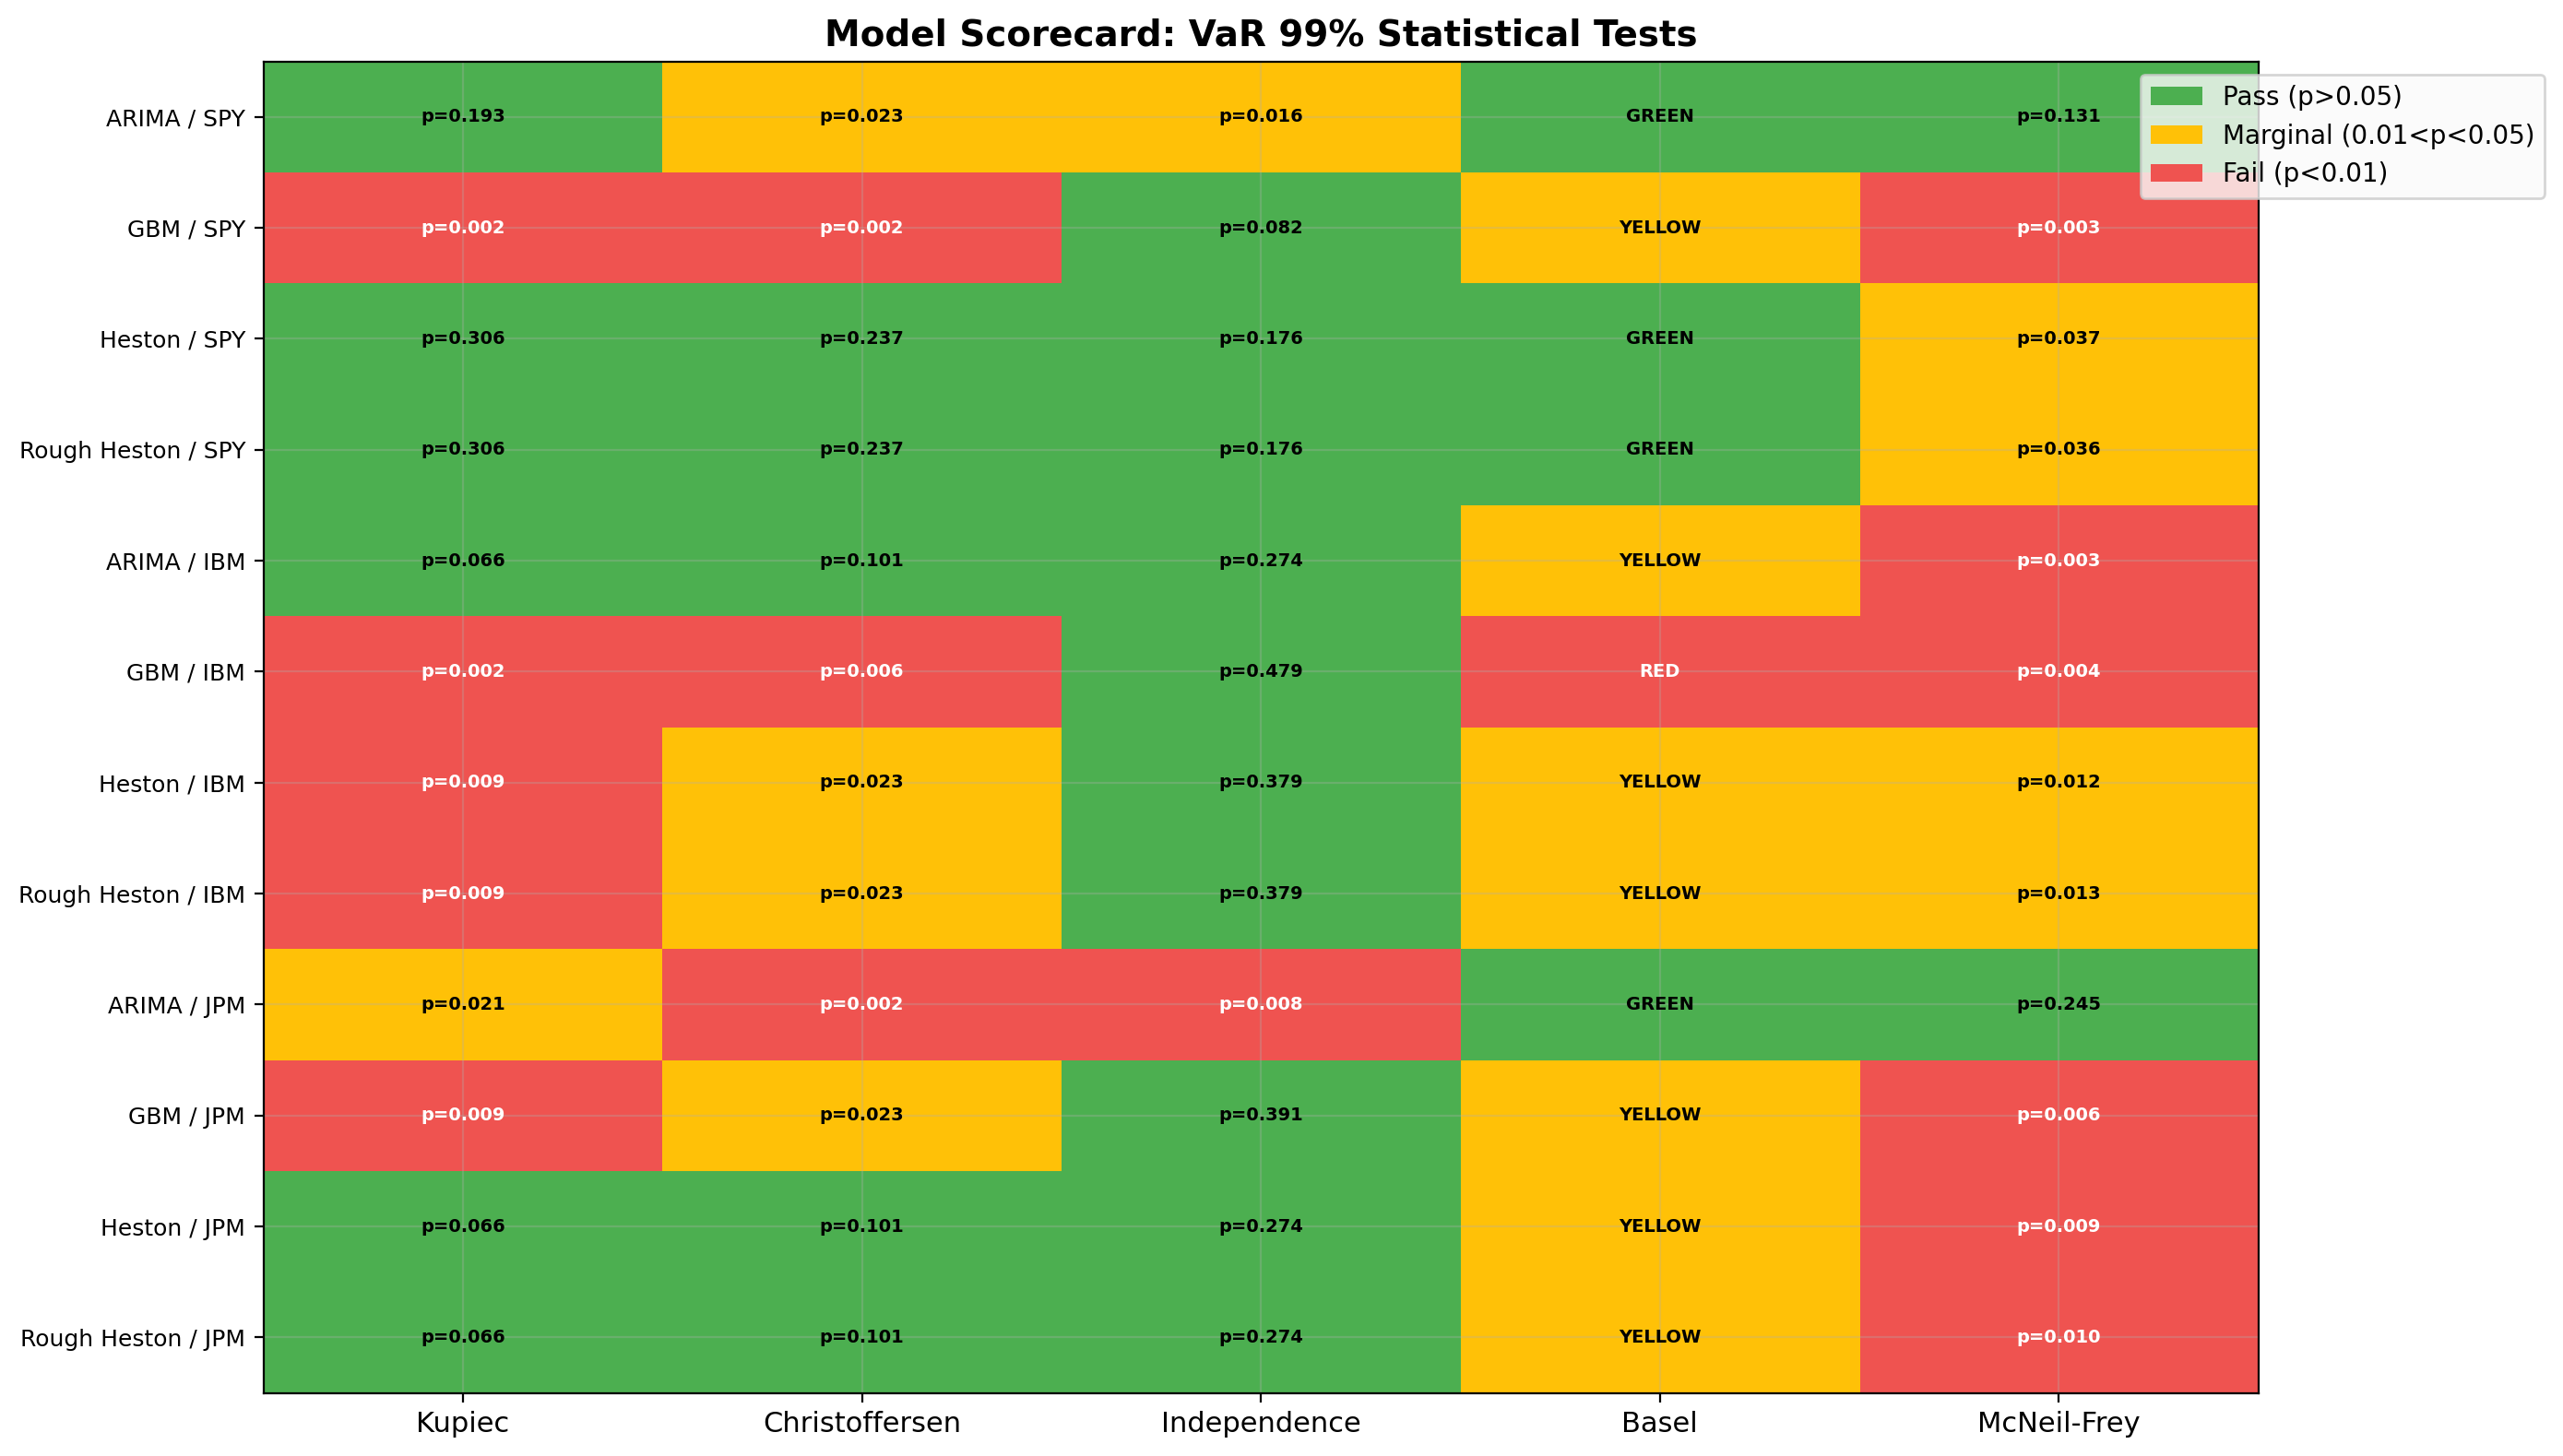
\includegraphics[width=0.95\textwidth]{figures/model_scorecard.png}
\caption{Model scorecard heatmap. Green cells indicate statistical test passage ($p > 0.05$); red cells indicate failure. Only Heston and Rough Heston achieve green across all tests at the 99\% confidence level.}
\label{fig:scorecard}
\end{figure}

% ===== SECTION 4 =====
\section{The Dollar Cost of Model Risk --- Dynamic Hedging}

The preceding sections quantify model risk in statistical terms---exceedance rates, $p$-values, percentage differences in ES. This section translates those abstractions into a concrete financial quantity: the profit-and-loss distribution of a hedged options position.

\subsection{Setup}

A trader sells a 3-month ATM call option on SPY ($S_0 = 100$, $K = 100$) and collects a Black--Scholes premium of \$4.62. The trader delta-hedges daily using the Black--Scholes formula with assumed constant volatility $\sigma = 0.20$:
\begin{equation}
\Delta_{\text{BS}} = N(d_1), \quad d_1 = \frac{\ln(S/K) + (r + \sigma^2/2)\,\tau}{\sigma\sqrt{\tau}}
\end{equation}

Under GBM (when the model is correct), the hedge is nearly perfect---the trader earns approximately the risk-free rate on the premium collected. Under stochastic volatility (when the model is \textit{wrong}), systematic hedge errors accumulate because the true delta depends on the instantaneous variance $v_t$, which the trader ignores.

\subsection{Results}

We simulate 100{,}000 hedge P\&L paths under three ``true'' market dynamics using calibrated SPY parameters:

\begin{table}[H]
\centering
\begin{tabular}{llcccc}
\toprule
\textbf{True Dynamics} & \textbf{Hedge Strategy} & \textbf{P\&L Std} & \textbf{ES$_{99}$} & \textbf{ES Ratio} & \textbf{$P$(loss $>$ 2$\times$)} \\
\midrule
GBM            & BS constant $\sigma$ & \$0.52 & \$0.90  & 1.0$\times$ & 0.00\% \\
Heston         & BS constant $\sigma$ & \$1.72 & \$5.53  & 6.1$\times$ & 0.06\% \\
Heston         & BS local vol         & \$1.74 & \$4.15  & 4.6$\times$ & 0.00\% \\
Rough Heston   & BS constant $\sigma$ & \$2.34 & \$10.42 & 11.6$\times$ & 0.55\% \\
Rough Heston   & BS local vol         & \$2.29 & \$7.63  & 8.5$\times$ & 0.11\% \\
\bottomrule
\end{tabular}
\caption{Hedge P\&L statistics per \$100 notional. ``ES Ratio'' is relative to the GBM baseline. Under Rough Heston, 0.55\% of paths produce losses exceeding twice the collected premium---a scenario the Black--Scholes framework considers impossible.}
\label{tab:hedging}
\end{table}

Under GBM, the hedge works as advertised: ES$_{99}$ is \$0.90, well within the \$4.62 premium collected. Under Heston, ES$_{99}$ jumps to \$5.53---a 6$\times$ increase that exceeds the premium. Under Rough Heston, where volatility is rough and harder to track, ES$_{99}$ reaches \$10.42---a 12$\times$ increase. The trader who assumes Black--Scholes is correct would set aside reserves for \$0.90 of tail risk; the actual tail risk is \$10.42.

On a \$10M notional position, this translates to a hidden tail risk of \$553{,}000--\$1{,}042{,}000 that the Black--Scholes-assuming trader does not see. This is not a hypothetical stress scenario---it is the expected 99th-percentile loss under empirically calibrated market dynamics.

Even a simple improvement---using $\sigma_t = \sqrt{v_t}$ (local volatility updated daily from recent realized variance) instead of constant $\sigma$---reduces Heston ES$_{99}$ from \$5.53 to \$4.15, a 25\% improvement. Under Rough Heston, local vol hedging reduces ES$_{99}$ from \$10.42 to \$7.63, a 27\% reduction. But the residual risk remains substantial: model risk cannot be hedged away entirely; it can only be acknowledged and managed.

\begin{figure}[H]
\centering
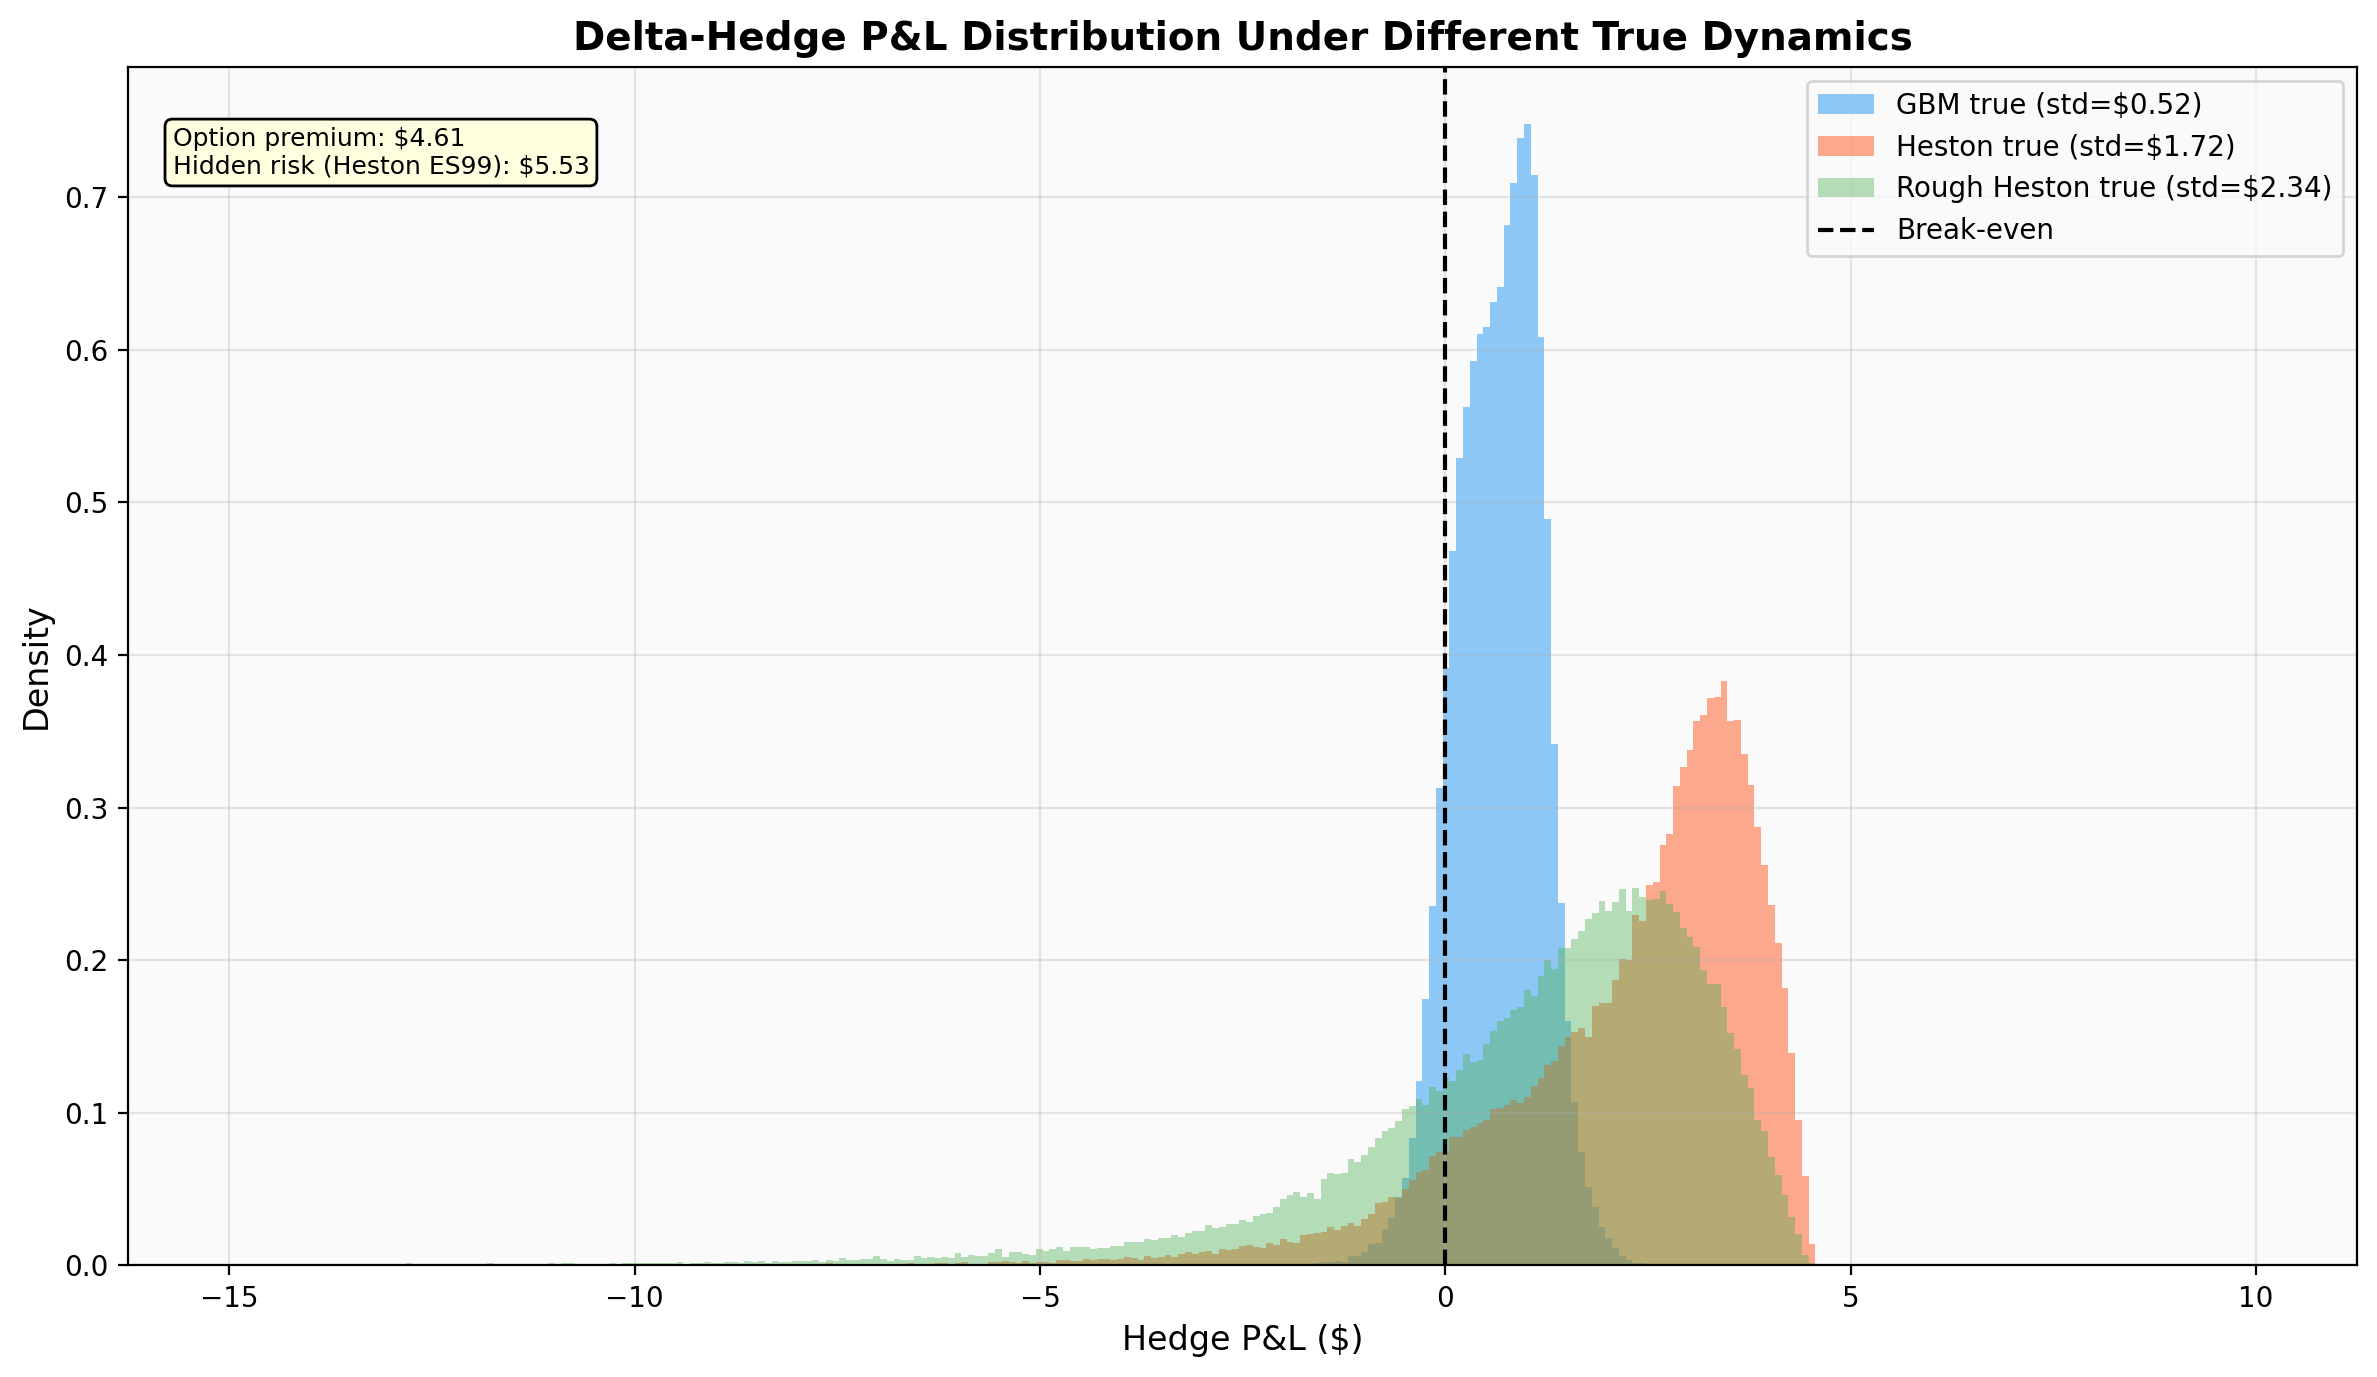
\includegraphics[width=0.95\textwidth]{figures/hedge_pnl_distributions.png}
\caption{Hedge P\&L distributions under three market dynamics. The Black--Scholes-assuming trader (blue) sees a tight distribution around zero. Under Heston (orange) and Rough Heston (red), the true P\&L develops heavy left tails that the trader does not anticipate.}
\label{fig:hedge_pnl}
\end{figure}

% ===== SECTION 5 =====
\section{Interactive Dashboard}

To make these results accessible beyond static figures, we built an interactive Streamlit dashboard deployed at \url{https://quantriskeng.streamlit.app}. The application provides five pages: a Model Explorer for real-time parameter adjustment with immediate visual feedback, a three-model risk comparison, portfolio risk analysis with copula-dependent tail scenarios, walk-forward backtest visualization with statistical test details, and dynamic hedging analysis with position scaling.

The dashboard uses a dual-mode architecture: locally, it connects to the C++/pybind11 simulation engine for full-speed Monte Carlo with up to 500{,}000 paths; on cloud deployment, it falls back to a pure Python simulation backend that supports any parameter combination interactively. All five pages render correctly in both modes, allowing reviewers and collaborators to explore the full risk engine without compiling C++ code.

% ===== SECTION 6 =====
\section{What We Learned}

Three findings stand out from this project, each with direct implications for how risk is managed in practice.

\textbf{Model risk is quantifiable and material.} The choice of volatility model changes ES$_{99}$ by 30\%. The choice of dependence model changes portfolio ES by 15\%. Combined, using GBM with a Gaussian copula instead of Heston with a vine copula underestimates tail risk by over 40\%. These are not edge cases or stress scenarios---they are the baseline estimates under empirically calibrated parameters.

\textbf{Prediction intervals, not point forecasts.} No model---ARIMA, Random Forest, XGBoost, or any stochastic volatility model---can reliably predict tomorrow's return. But stochastic volatility models can produce calibrated prediction intervals that contain the true value at the stated confidence level. Our backtest confirms this: Heston passes both Kupiec and Christoffersen tests on 1{,}053 days of real SPY data, achieving Basel GREEN where GBM fails. Risk management does not need accurate point forecasts; it needs honest uncertainty quantification.

\textbf{Model risk has direct financial consequences.} A trader delta-hedging with Black--Scholes faces 6--12$\times$ more tail risk than the model predicts. On a \$10M position, this is a hidden exposure of \$553K--\$1.04M. This is not an academic curiosity; it is a P\&L line item that materializes during crises---precisely when institutions can least afford unexpected losses.

\textbf{What's next.} CUDA GPU acceleration for nested Monte Carlo---computing the distribution of ES itself, quantifying estimation uncertainty as meta-risk. Calibration on implied volatility surfaces for production-quality parameter estimation. The code is open-source at \url{https://github.com/notgabrielpop/quant-risk-engine}, and the interactive dashboard is live at \url{https://quantriskeng.streamlit.app}.

The question was never ``What will the price be?'' The question is ``What does the full landscape of possibilities look like, how confident are we in our map, and what does it cost when the map is wrong?''

% ===== REFERENCES =====
\vspace{1em}
\hrule
\vspace{0.5em}

\begin{thebibliography}{12}

\bibitem{heston1993}
S.~L. Heston, ``A closed-form solution for options with stochastic volatility with applications to bond and currency options,'' \textit{The Review of Financial Studies}, vol.~6, no.~2, pp.~327--343, 1993.

\bibitem{gatheral2018}
J.~Gatheral, T.~Jaisson, and M.~Rosenbaum, ``Volatility is rough,'' \textit{Quantitative Finance}, vol.~18, no.~6, pp.~933--949, 2018.

\bibitem{andersen2008}
L.~Andersen, ``Simple and efficient simulation of the Heston stochastic volatility model,'' \textit{Journal of Computational Finance}, vol.~11, no.~3, pp.~1--42, 2008.

\bibitem{cont2001}
R.~Cont, ``Empirical properties of asset returns: stylized facts and statistical issues,'' \textit{Quantitative Finance}, vol.~1, no.~2, pp.~223--236, 2001.

\bibitem{mcneil2015}
A.~J. McNeil, R.~Frey, and P.~Embrechts, \textit{Quantitative Risk Management: Concepts, Techniques and Tools}, revised ed. Princeton University Press, 2015.

\bibitem{glasserman2003}
P.~Glasserman, \textit{Monte Carlo Methods in Financial Engineering}. Springer, 2003.

\bibitem{joe2010}
S.~Joe and F.~Y. Kuo, ``Constructing Sobol sequences with better two-dimensional projections,'' \textit{SIAM Journal on Scientific Computing}, vol.~30, no.~5, pp.~2635--2654, 2008.

\bibitem{aas2009}
K.~Aas, C.~Czado, A.~Frigessi, and H.~Bakken, ``Pair-copula constructions of multiple dependence,'' \textit{Insurance: Mathematics and Economics}, vol.~44, no.~2, pp.~182--198, 2009.

\bibitem{kupiec1995}
P.~Kupiec, ``Techniques for verifying the accuracy of risk measurement models,'' \textit{The Journal of Derivatives}, vol.~3, no.~2, pp.~73--84, 1995.

\bibitem{christoffersen1998}
P.~F. Christoffersen, ``Evaluating interval forecasts,'' \textit{International Economic Review}, vol.~39, no.~4, pp.~841--862, 1998.

\bibitem{mcneil2000}
A.~J. McNeil and R.~Frey, ``Estimation of tail-related risk measures for heteroscedastic financial time series: an extreme value approach,'' \textit{Journal of Empirical Finance}, vol.~7, no.~3--4, pp.~271--300, 2000.

\bibitem{sklar1959}
A.~Sklar, ``Fonctions de r\'{e}partition \`{a} $n$ dimensions et leurs marges,'' \textit{Publications de l'Institut de Statistique de l'Universit\'{e} de Paris}, vol.~8, pp.~229--231, 1959.

\end{thebibliography}

\end{document}
